\documentclass[12pt]{article}

\usepackage{amsthm}
\usepackage{amsmath}
\usepackage{amssymb}
\usepackage{amsfonts}

\usepackage{scicite}

\usepackage{times}

\usepackage{graphicx}

\topmargin 0.0cm
\oddsidemargin 0.2cm
\textwidth 16cm 
\textheight 21cm
\footskip 1.0cm

\newenvironment{sciabstract}{%
\begin{quote} \bf}
{\end{quote}}

\title{Predicting the long-term impact of AI assistants on collective intelligence}

\author
{Jaeseung Kim,$^{1}$ Sang Woo Park,$^{1,2,\ast}$
\\
\normalsize{$^{1}$School of Biological Sciences, Seoul National University,}\\
\normalsize{Seoul, Korea}\\
\normalsize{$^{2}$Institute for Data Innovation in Science, Seoul National University, Seoul, Korea,}\\
\normalsize{Seoul, Korea}\\
\\
\normalsize{$^\ast$To whom correspondence should be addressed; E-mail: sangwoopark@snu.ac.kr.}
}

\date{}

\begin{document} 

\baselineskip24pt

\maketitle 

\begin{sciabstract}
Artificial intelligence (AI) assistants can improve individual performance, but they can also weaken unaided performance and limit interest diversity, raising questions about their long-term effects on collective intelligence (CI).
To address this question, we develop an evolutionary model in which individuals participate in prediction tasks, consult AI, and imitate better-performing peers.
Classic incentives that promote CI without AI can fail under ``Chatbot AI'', whose predictions depend on users’ interests, by reducing interest diversity or propagating systematic AI bias. 
Directly rewarding or penalizing AI use does not reliably mitigate these effects. 
Instead, a balanced incentive that preserves minority expertise and rewards contributions to collective accuracy promote CI under Chatbot AI, while an additional incentive restores unaided collective accuracy.
\end{sciabstract}

\section*{Introduction}

Collective intelligence (CI) describes a phenomenon in which a group’s ability to solve problems, make decisions, or adapt to changing environments exceeds each member’s ability \cite{galton1907vox,lorge1958survey,yaniv2007using,woolley2010evidence,hommes2005coordination}.
This phenomenon, also referred to as wisdom of crowds, has thus served as a central mechanism underlying the success of diverse organizations, ranging from animal groups \cite{dreyer2025comparing,simons2004many,berdahl2013emergent} and human societies \cite{woolley2010evidence, riedl2021quantifying} to machine-learning systems \cite{breiman1996bagging,breiman2001random}.
Understanding the conditions that promote and maintain CI therefore remains a fundamental question across social sciences \cite{mann2017optimal}, evolutionary biology \cite{wang2025individual}, and computer science \cite{werfel2026fluid}.
Addressing this question has become particularly timely as artificial intelligence (AI) has begun to reshape how individuals acquire information, make decisions, and contribute to collective outcomes \cite{cui2024ai}.

The recent emergence of generative AI and large language models (LLMs) has changed the way individuals engage in various cognitive tasks, ranging from everyday tasks \cite{noy2023experimental,brynjolfsson2025generative} to scientific discovery \cite{lu2026towards} and creative writing \cite{doshi2024generative}.
In particular, while the use of generative AI models, such as ChatGPT, has been rapidly increasing \cite{bick2026rapid,sajadieh2026artificial}, the potential long-term impact of AI assistants on human society, especially CI, remains uncertain.
Some argue that AI can promote CI by enhancing individual expertise \cite{vaccaro2024combinations} and opinion aggregation \cite{burton2024large,tessler2024ai}.
Conversely, empirical evidence indicates that the use of AI can limit the diversity of opinions \cite{ fugener2021will,doshi2024generative,lee2024empirical,meincke2025chatgpt}, a key requirement for the emergence of CI \cite{hong2004groups,lorenz2011social,aplin2014individual,becker2017network}.
We expect these AI-driven changes to shape long-term social evolution because successful individuals can influence which interests, beliefs, and patterns of AI use become prevalent in a population.

However, our ability to predict the long-term impact of AI assistants on human CI is hampered by the apparent discrepancy in the incentives that shape AI use.
On one hand, many industrial sectors are pushing towards increased AI use, where the number of ``tokens'' used is often perceived as a proxy for productivity \cite{bousquette2026tokenmaxxing,keary2026cult}.
On the other hand, many academic institutions appear to discourage AI use, reflecting concerns about plagiarism, misinformation, and limited independence \cite{thorp2023chatgpt,chawla2026researchers}.
Such discrepancy raises a question about whether directly incentivizing or penalizing AI use will benefit or harm human CI.
More broadly, previous work identified incentive structures that promote CI through social learning  \cite{wang2025individual}, but it remains unclear whether these structures remain effective in the presence of AI assistants.
Thus, a key challenge is to identify robust incentive structures that retain the benefits of AI while limiting risks such as the loss of diversity in individual opinions, thereby allowing for the maintenance of CI under AI use.

To address these questions, we extend previous approaches for modeling CI, in which each individual participates in a prediction task \cite{hong2012incentives,mann2017optimal,wang2025individual}.
Previous work modeled the prediction target $Y$ as a linear combination of underlying causal factors, $X_1, X_2, \dots, X_M$, (Fig. 1A) and assumed that each individual makes an independent prediction from a single observed factor of their interest $e_A$ and their belief $c_A$: $Y_A = c_A X_{e_A}$ (Fig. 1B).
Here, we further allow each individual to independently consult with AI assistants, which can also make their own predictions $Y_A^{AI}$, and revise their predictions by taking the weighted average according to their reliance on AI $\beta_A$: $Y_A^{\mathrm{re}} = \beta_A Y_A^{\mathrm{AI}} + (1-\beta_A)Y_A$ (Fig. 1B).
In doing so, we consider two forms of AI: Omniscient AI constructs predictions using all causal factors, whereas Chatbot AI responds only about the factor that the user is interested in (Fig. 1B).
These AI predictions can include both systematic biases and stochastic errors (Fig. 1B).
Then, these revised predictions are aggregated to form a collective prediction $\hat{Y}^{\mathrm{re}}$, which is then used to evaluate the collective accuracy of the population \cite{wang2025individual}: $1-\mathbb{E}[(Y-\hat{Y}^{\mathrm{re}})^2]/\mathbb{E}[(Y-\alpha_0)^2]$.
For Omniscient AI, we simply average revised predictions. 
For Chatbot AI, we average within interests and sum across represented interests.
Hereafter, we say that CI emerges when the collective accuracy reaches a near perfect level.

\begin{figure}[!th]
\includegraphics[width=\textwidth]{../Figures/Figure 1.pdf}
\caption{
\textbf{A schematic diagram of the model for individual and collective prediction in the presence of AI assistants.}
(A) The prediction target is modeled as a linear combination of causal factors.
(B) Each player is characterized by three strategies: interest, belief, and reliance on AI.
Players make predictions based on their interests and beliefs and subsequently revise them with AI assistance.
We consider two types of AI, Chatbot AI and Omniscient AI, which differ in the amount of information available for generating predictions.
(C) Players receive payoffs according to the incentive structure, and the population evolves through imitation of peers with higher payoffs.
}
\end{figure}

Individuals receive payoffs $\pi_A$ based on their performance and imitate the interests, beliefs, and AI reliance of peers with higher expected payoffs, allowing the population to evolve over time (Fig. 1C).
Following previous work \cite{wang2025individual}, we consider two incentive structures, which allow CI to emerge in the absence of AI.
First, the feedback structure gives higher payoffs to individuals whose predictions are aligned with the collective prediction error, rather than directly rewarding individual predictive accuracy: $\pi_A = Y_A^{\mathrm{re}}(Y-\hat{Y}^{\mathrm{re}})$.
Second, the niche-expert structure gives higher payoff to individuals who have both better predictive accuracy and a minority interest: $\pi_A = -\rho_{e_A}(Y_A^{\mathrm{re}}-Y)^2$, where $\rho_{e_A}$ represents the proportion of individuals sharing the same interest.
We assume that prediction events occur on a substantially faster timescale than social learning, which allow us to calculate the expected payoff $\mathbb{E}[\pi_A]$ of each player analytically and simulate social learning.
Full details of the model and derivations of the collective prediction, expected payoffs, and collective accuracy under the two AI models are provided in Materials and Methods as well as Supplementary Text.

We begin by characterizing the dynamics of CI with AI under two classic incentive structures from prior work \cite{wang2025individual}.
We show that the outcome depends on the information available to AI: Omniscient AI can preserve or improve collective accuracy, whereas Chatbot AI can undermine CI by limiting interest diversity or propagating systematic AI bias. 
Directly incentivizing or penalizing AI use fails to correct these effects and can further reduce collective accuracy.
Finally, we leverage these findings to propose a balanced incentive structure that preserves minority expertise while rewarding contributions to collective accuracy, thereby restoring CI under Chatbot AI. 
However, even when AI-assisted CI is restored, the population’s unaided collective accuracy remains suboptimal, requiring additional incentives that explicitly preserve unaided predictive ability.

\section*{Classic incentive structures for collective intelligence can fail under Chatbot AI}

\begin{figure}[!th]
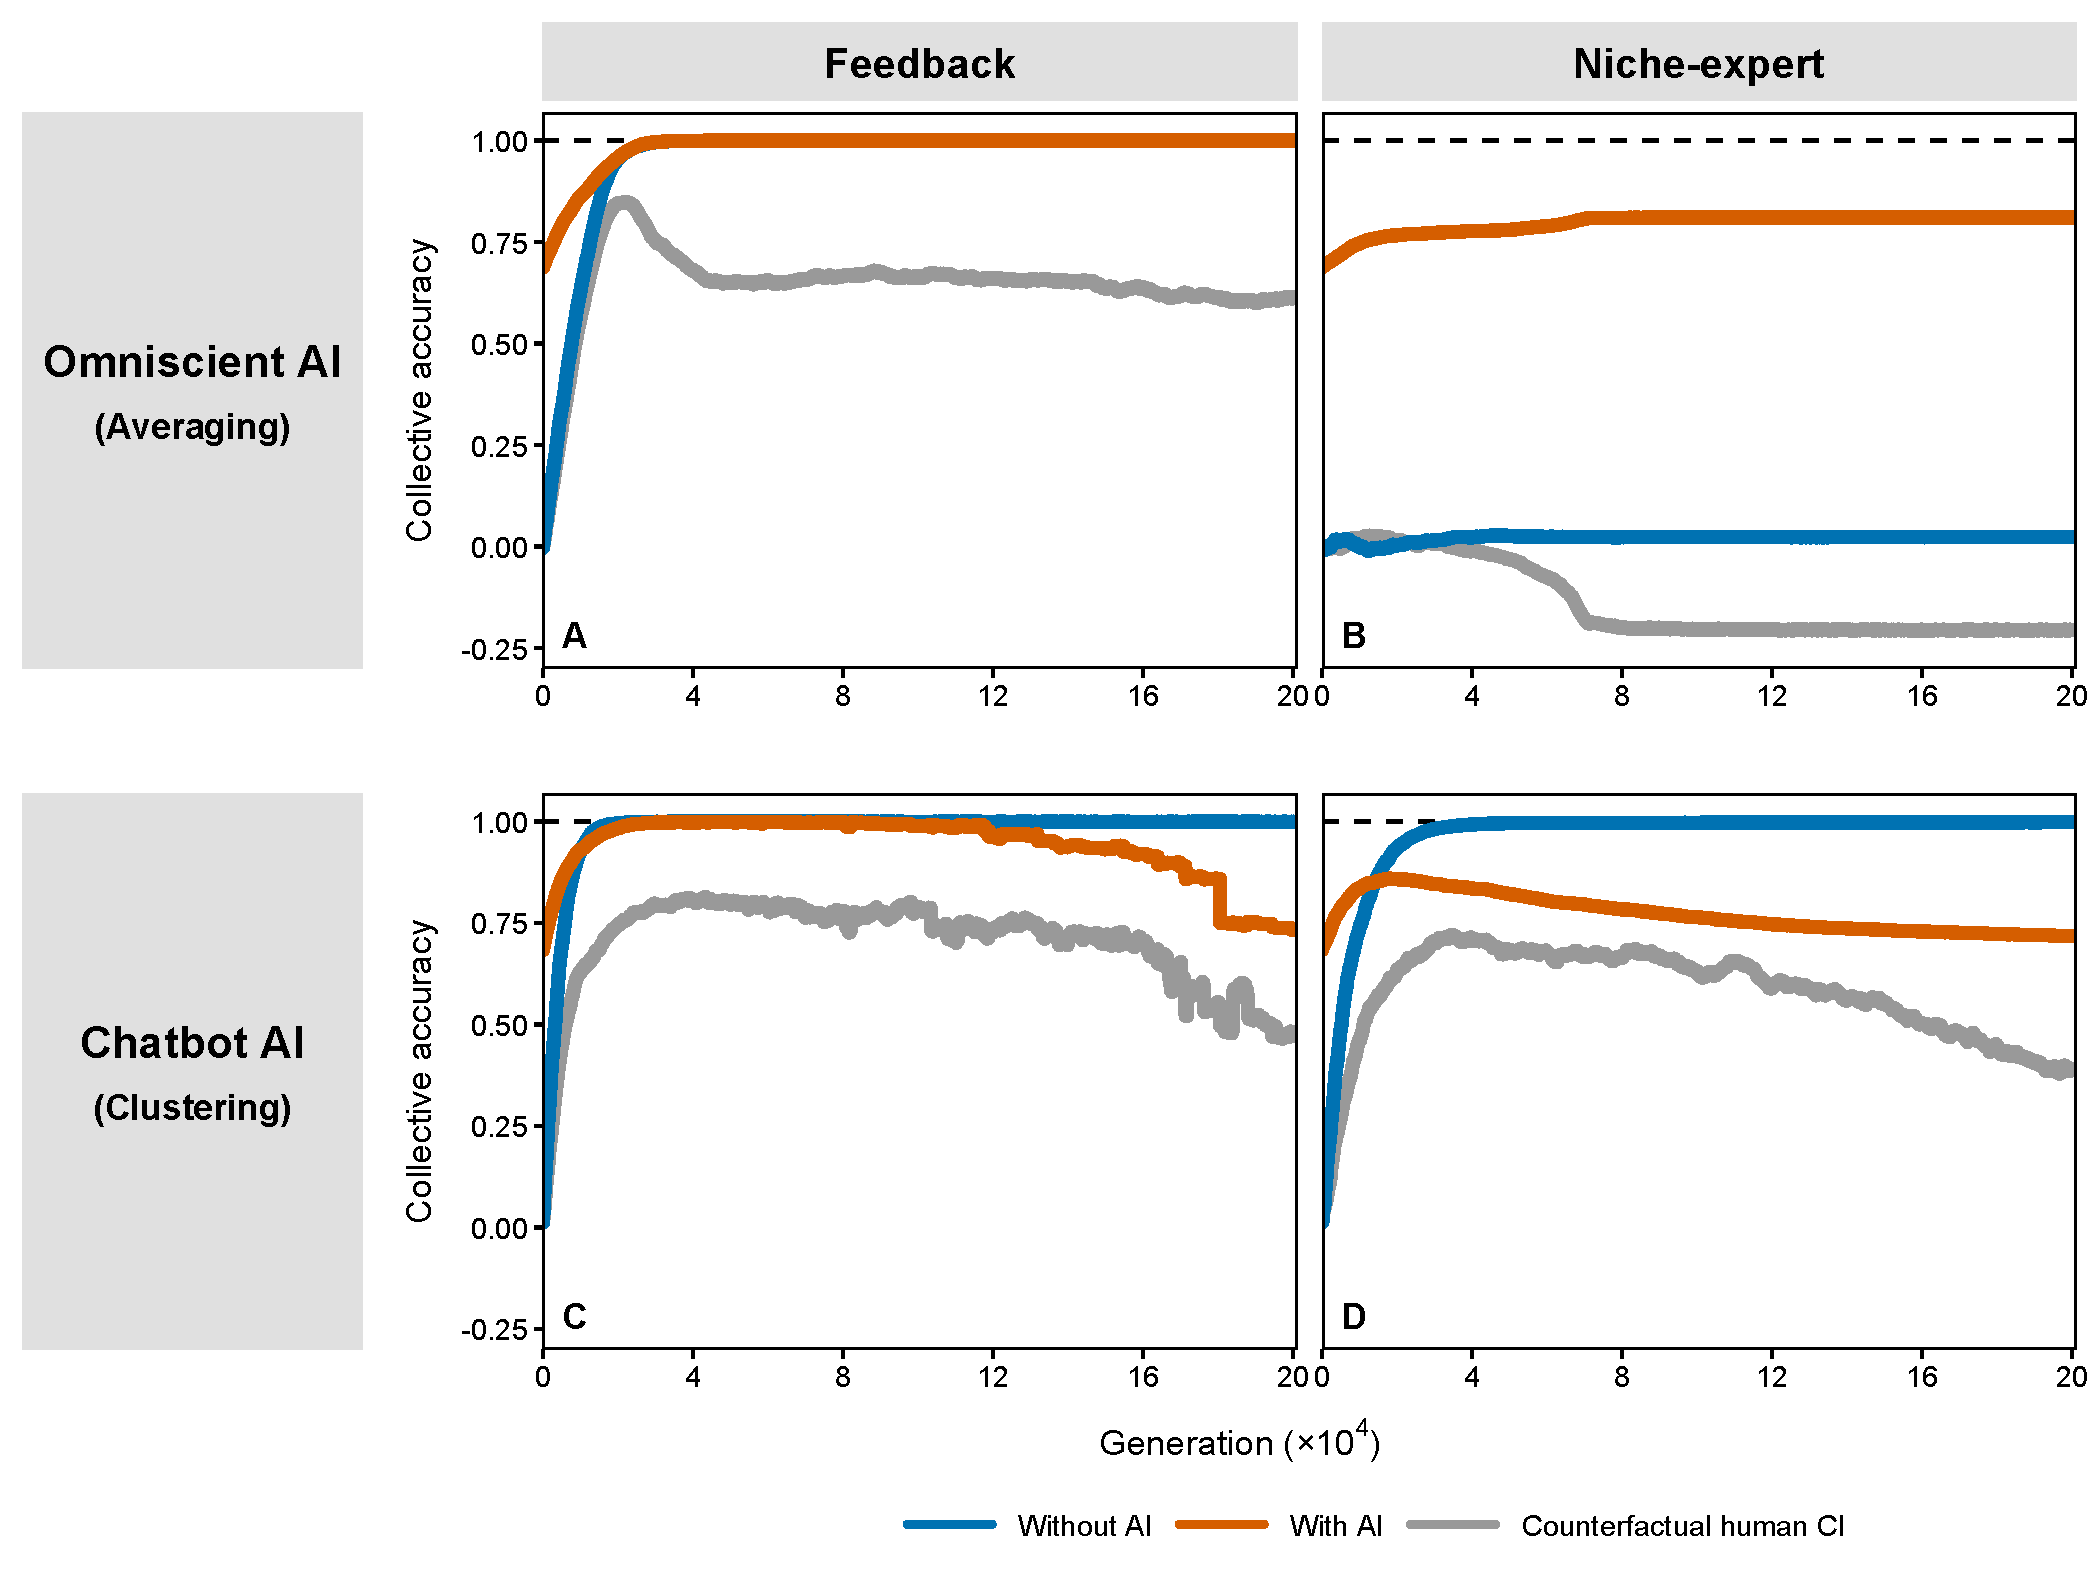
\includegraphics[width=\textwidth]{../Figures/Figure 2.pdf}
\caption{
\textbf{Comparison of collective accuracy with and without AI.} 
Trajectories of collective accuracy when the group is assisted by the Omniscient AI (A,B) and Chatbot AI (C,D).
Here, feedback (A,C) and niche-expert (B,D) incentive structures are considered.
Blue lines represent trajectories of collective accuracy without AI assistance.
Orange lines represent trajectories of collective accuracy with AI assistance.
Gray lines represent trajectories of counterfactual collective accuracy, computed from players’ unrevised predictions, indicating the group’s predictive accuracy if AI assistance were unavailable at the given generation.
Prediction target parameters: $M = 50$, $\alpha_i \sim U(-5, 5)$, and $\sigma_i \sim U(0, 3)$.
Evolutionary parameters: $s = 50$ and $\mu = 0$.
Population parameters: $N = 10{,}000$, $c_A \sim \mathcal{N}(0, 100^2)$ for (A, B), $c_A \sim \mathcal{N}(0, 5^2)$ for (C, D), and $\beta_A \sim U(0, 1)$. 
AI parameters: $b_i = 0.4$ and $\tau = 0.3$.
}
\end{figure}

First, consistent with \cite{wang2025individual}, previously proposed incentive structures allow collective intelligence to emerge in the absence of AI (Fig. 2A,C,D).
One exception is the use of simple averaging with niche-expert incentive structures, under which the collective accuracy of the population remains near zero.
This is because each individual accurately predicts the contribution of their factor of interest, but averaging these partial predictions dilutes the factor-specific contributions instead of reconstructing the full prediction target (Fig. S1).

The use of Omniscient AI can either preserve CI under the feedback incentive structure (Fig. 2A) or promote higher collective accuracy under the niche-expert incentive structure (Fig. 2B). 
These results are robust across different levels of AI accuracy (Fig. S2) and can also be characterized analytically in the large-population limit (Supplementary Text).

Under the feedback incentive structure, the use of Chatbot AI leads to a loss of diversity in the population's interest, making it impossible to account for effect of some causal factors (Fig. S2, S3).
This causes an increase in collective variance and a stochastic decrease in collective accuracy (Fig. 2C; Fig. S3).
We note that the loss of interest diversity may arise even in the absence of AI in finite populations (Fig. S3), but the use of Chatbot AI makes the group more vulnerable to such loss (Fig. S4).
Under the niche-expert incentive structure, the population becomes overly reliant on AI, causing the collective prediction to inherit the AI's bias (Fig. S3).
This leads to an increase in collective bias and a decrease in collective accuracy (Fig. 2; Fig. S3).
Interestingly, the niche-expert structure can instead reduce reliance on AI when the target intercept, $\alpha_0$, and AI bias have opposite signs (Figs. S2,S5).
In this case, the population reduces its reliance on AI assistance, allowing CI to emerge eventually. 
However, the emergence of CI can be substantially delayed compared with the population without AI (Fig. S5).

To investigate whether the group can retain its predictive ability when AI assistance suddenly becomes unavailable, we quantify counterfactual collective accuracy based on unrevised predictions, retaining the population’s evolved interests and beliefs. 
Across all scenarios, counterfactual collective accuracy is lower than the accuracy of the corresponding AI-assisted population and the accuracy of populations that evolved without AI (Fig. 2).
Thus, the accuracy achieved with AI assistance does not necessarily reflect the population’s ability to make equally accurate predictions without it.

\section*{Directly incentives and penalties for AI do not reliably improve collective accuracy}

\begin{figure}[!th]
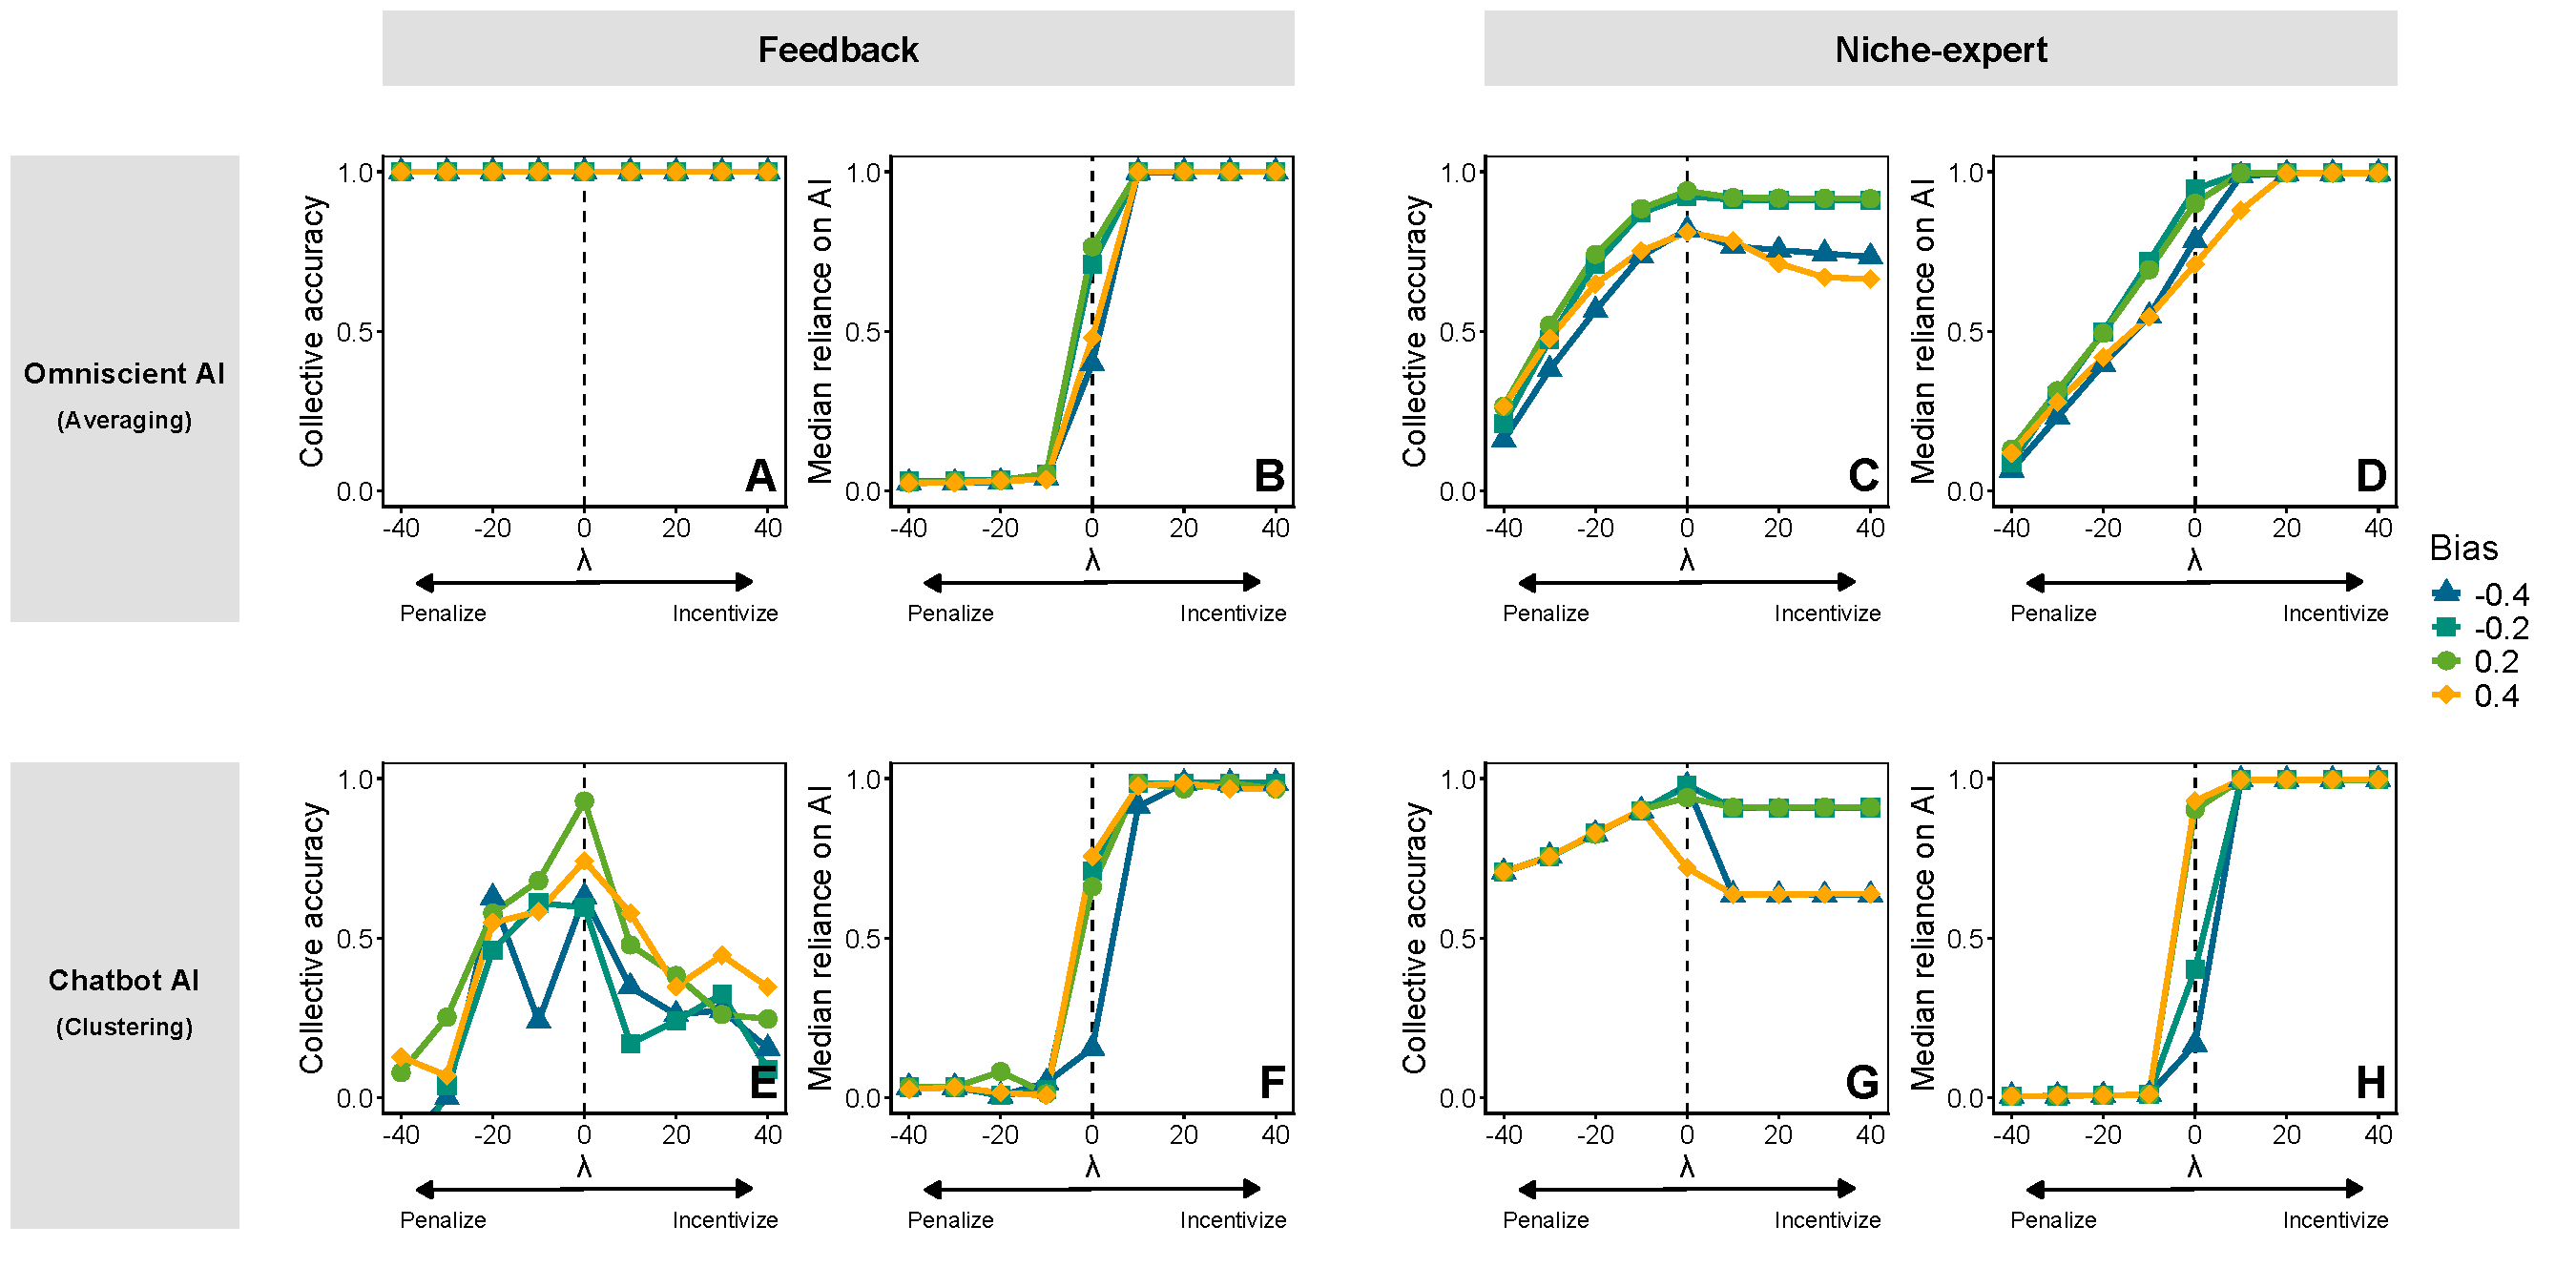
\includegraphics[width=\textwidth]{../Figures/Figure 3.pdf}
\caption{
\textbf{Collective accuracy under the influence of direct intervention on AI use.}
Collective accuracy and median reliance on AI under varying strengths of intervention ($\lambda$) across different assumptions about AI types (Omniscient AI, A--D and Chatbot AI, E--H) and incentive structures (Feedback, A,B,E,F, and Niche expert, C,D,G,H).
Positive $\lambda$ represents an incentive for AI use, whereas negative $\lambda$ represents a penalty for AI use.
In each panel, the vertical dashed line indicates the original incentive structure ($\lambda = 0$).
Four AI bias levels are shown: $b_i = \pm 0.2$, representing higher-accuracy AI, and $b_i = \pm 0.4$, representing lower-accuracy AI.
Collective accuracy (A,C,E,G) and median reliance on AI (B,D,F,H) are averaged over generations 190,000--200,000.
Prediction target parameters: $M = 50$, $\alpha_i \sim U(-5, 5)$, and $\sigma_i \sim U(0, 3)$.
Evolutionary parameters: $s = 50$ and $\mu = 0$.
Population parameters: $N = 10{,}000$, $c_A \sim \mathcal{N}(0, 100^2)$ for (A--D), $c_A \sim \mathcal{N}(0, 5^2)$ for (E--H), and $\beta_A \sim U(0, 1)$. 
AI parameter: $\tau = 0.3$.
}
\end{figure}

Given the strong influence of AI on collective outcomes, a straightforward intervention is to directly incentivize or penalize the use of AI. 
To investigate whether such direct incentives or penalties can promote CI, we modify the two incentive structures by adding a payoff term proportional to individual reliance on AI:
\begin{equation}
\mathrm{Feedback /} \mathrm{Niche\text{-}expert} + \lambda \beta_A
\end{equation}
where $\lambda$ represent the strength of intervention ($\lambda > 0$) or penalty ($\lambda < 0$), and $\beta_A$ represent individual reliance on AI (Supplementary Text).

We find that direct incentives and penalties on AI use do not consistently improve collective accuracy (Fig. 3).
When Omniscient AI is used under the feedback structure, the population retains collective intelligence regardless of the intervention strength (Fig. 3A), despite large changes in reliance on AI (Fig. 3B).
In other scenarios, directly incentivizing or penalizing AI use causes individuals to imitate others based on their AI use rather than their predictive accuracy (Fig. 3C,E,G).
When AI bias is relatively large, a weak penalty can lead to higher collective accuracy, but this improvement is restricted to a narrow parameter regime (Fig. 3G).
Overall, these results indicate that directly rewarding or penalizing AI use may exacerbate rather than mitigate its effects on collective accuracy.

\section*{Balanced incentives promote collective intelligence with AI}

\begin{figure}[!th]
\begin{center}
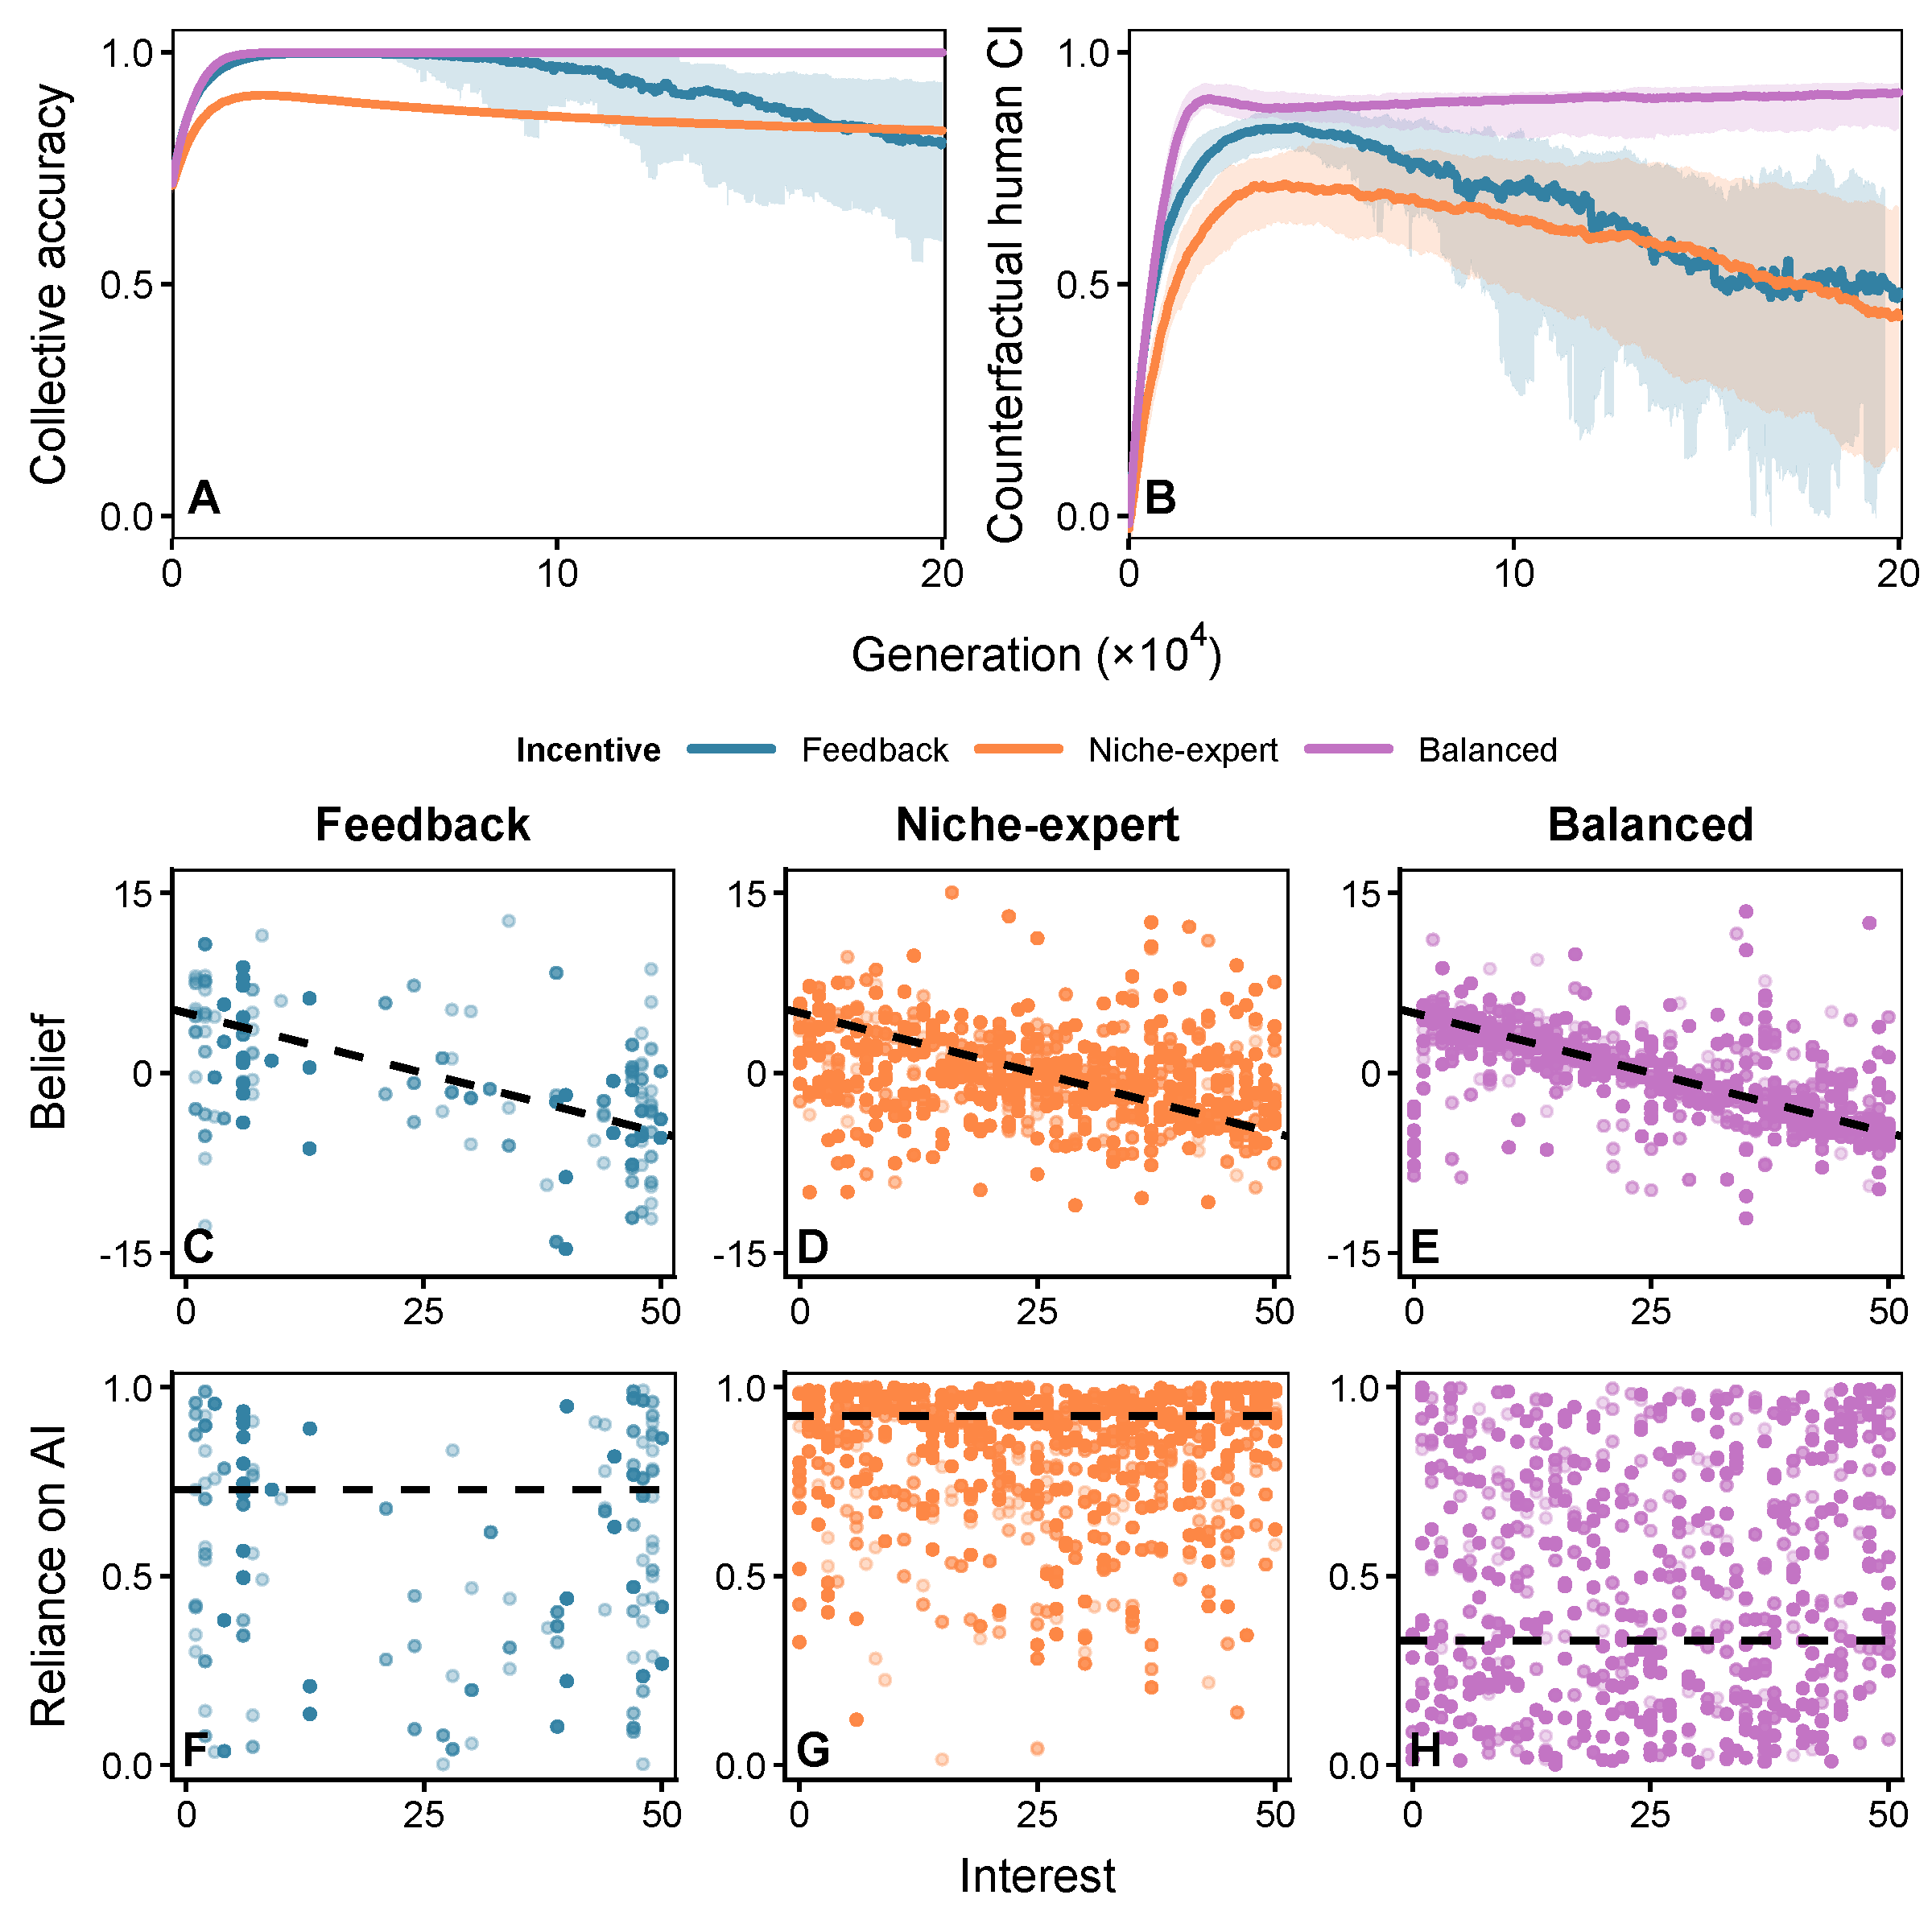
\includegraphics[width=0.9\textwidth]{../Figures/Figure 4.pdf}
\caption{
\textbf{Balanced structure can promote collective intelligence.} 
Trajectories of collective accuracy (A) and counterfactual human CI (B) under three incentive structures (feedback, niche-expert, and balanced) with Chatbot AI.
Distributions of individual interest and belief (C-E) and of interest and reliance on AI (F-H) after 200,000 generations. 
Each point represents an individual. 
Dashed lines in panels C-E represent the true coefficients ($\alpha_i$) of the prediction target.
Dashed horizontal lines in panels F-H indicate the median reliance on AI.
Prediction target parameters: $M = 50$, $\alpha_i = 5 - 0.2i$, and $\sigma_i \sim U(0, 3)$. 
Evolutionary parameters: $s = 50$ and $\mu = 0$.
Population parameters: $N = 10{,}000$, $c_A \sim \mathcal{N}(0, 5^2)$, and $\beta_A \sim U(0, 1)$. 
AI parameters: $b_i = 0.4$ and $\tau = 0.3$.
}
\end{center}
\end{figure}

The contrasting failures of the feedback and niche-expert structures suggest combining their complementary roles.
Here, we propose a ``balanced'' incentive structure, modeled as the average of the feedback and niche expert incentives (Supplementary Text).

The core idea behind the balanced structure is to maintain interest diversity and prevent collective bias.
On one hand, the feedback incentive structure is prone to the loss of interest diversity but can prevent collective bias by rewarding predictions aligned with the collective prediction error.
On the other hand, the niche-expert structure can maintain interest diversity because it directly incentivizes minority interests.
However, it does not directly reward the correction of collective bias, because individuals sharing the same interest are rewarded according to their individual predictive performance.

Therefore, when the two incentive structures are combined, the population achieves CI by maintaining interest diversity while limiting collective bias (Fig. 4A; Fig. S6).
Under the balanced structure, individuals remain more evenly distributed across causal factors, and their beliefs lie closer to the true coefficients than under either incentive structure alone (Fig. 4C--E). 
The balanced structure also produces higher counterfactual collective accuracy than the feedback or niche-expert structure (Fig. 4B; Fig. S6).
These patterns are robust to balancing weights (Fig. S7), and are driven by the emergent property of the balanced structure, under which the population increases its reliance on AI as AI becomes more accurate (Fig S8).


\section*{Discussion}

The ongoing race towards the development of ``better'' AI continues to pose questions about the societal benefits and risks of AI use \cite{bender2021dangers,burton2024large,cui2024ai}.
Here, we used mathematical models of evolutionary dynamics to investigate how AI use and incentive structures jointly affect the emergence of CI.
We find that an ``Omniscient'' AI model, which incorporates information about all relevant causal factors, can improve collective accuracy, whereas a ``Chatbot'' AI model, whose outcome depends on the user's interest, can impair it.
These contrasting outcomes arise because AI assistance affects not only individual predictions, but also the population's interest diversity, beliefs, and reliance on AI.
We also show that directly incentivizing or penalizing AI use, independent of individual's performances, can further limit the collective accuracy of the population. 
Instead, a balanced incentive structure can maintain CI by promoting diversity and limiting bias.

Our analysis reveals that AI can prevent the emergence of CI through two different mechanisms.
First, AI use can cause individuals to concentrate on a subset of the factors that determine the prediction target, thereby reducing diversity in their interests.
This result is broadly consistent with recent empirical studies showing that AI assistance can improve individual performance but limit the diversity of outputs, in domains ranging from scientific research \cite{hao2026artificial} to creative writing \cite{doshi2024generative}.
Second, over-reliance on AI can cause the population to inherit inherent biases in AI's predictions \cite{fugener2021will,vicente2023humans}, causing the prediction accuracy to decrease eventually.
This mechanism can prevent the emergence of CI even when the interest diversity is maintained because biases in AI predictions can be amplified when individual predictions are aggregated.
Thus, preserving the diversity of ideas will not be sufficient to promote CI.
Instead, AI use need to be calibrated to prevent systematic AI biases from becoming collective biases \cite{buccinca2021trust}.

Our analysis of counterfactual collective accuracy also raises an important concern for future AI use:
while AI use may improve the apparent performance of individuals and, in some cases, the population as a whole, it can simultaneously reduce the population’s ability to make accurate predictions without AI. 
These results echo findings from a recent field experiment, which demonstrated that students, who seemingly performed better in solving mathematics problems under AI assistance, performed worse on their own than those who did not have access \cite{bastani2025generative}.
These findings highlight the need to evaluate AI tools not only by the performance gains they provide during use, but also by whether individuals and populations retain the ability to perform without them \cite{melumad2025experimental,ke2026ai}.
Making this distinction clear will be particularly important for education, where AI may help students complete a task without helping them learn how to do it on their own \cite{bastani2025generative,melumad2025experimental}.

As generative AI and large language models are already generating substantial benefits, many organizations, both industrial and academic, are increasingly seeking to improve their collective performance by regulating AI use \cite{thorp2023chatgpt,bousquette2026tokenmaxxing,chawla2026researchers,keary2026cult}.
Such regulations may take direct forms, including AI-use policies or token-based leaderboards, or may operate indirectly through other incentives, such as productivity rewards or the social stigma associated with AI use \cite{reif2025evidence}.
Our model suggests that directly incentivizing or penalizing AI use is unlikely to induce appropriately calibrated reliance on AI or to promote CI.
Incentivizing AI use could lead to overreliance, causing groups to propagate AI biases, whereas penalizing AI use could lead to underreliance, preventing groups from using AI even when it performs well in the relevant domain.
Our result instead shows that appropriate AI use and accurate CI can be promoted by focusing on the traditional properties of groups that have been emphasized for decades:
maintaining diversity and preventing collective bias, rather than on AI use itself \cite{hong2004groups,lorenz2011social,mann2017optimal}.

There are several limitations to our analyses.
First, our model allows for social learning among humans, but AI's inherent ability remains fixed throughout the evolutionary process.
In reality, AI can also learn from human-generated data \cite{ouyang2022training}.
Such bidirectional learning could increase the similarity between human and AI errors and thereby reduce group performance \cite{glickman2025human}.
Second, we model AI errors using fixed, factor-specific additive biases and independent random errors.
This assumption allows random errors to be reduced through aggregation, while systematic biases can still persist in the collective prediction.
In reality, AI errors may have more complex structures, including biased estimates of factor effects and correlated errors across individuals, factors, or repeated interactions.
Further empirical and theoretical work is therefore needed to understand how these error structures affect the emergence of CI.
Finally, following established models of CI, we assume that the prediction target is a linear combination of independent causal factors.
This assumption does not hold for many real-world tasks, where causal factors may be correlated or interact nonlinearly.
Future studies should therefore investigate how nonlinear relationships between causal factors and prediction targets affect the interaction between AI assistance and the emergence of CI.

The rapid adoption of AI assistants is changing how individuals learn, work, and make decisions \cite{tessler2024ai,glickman2025human,sajadieh2026artificial,bick2026rapid,ke2026ai}.
While the immediate benefits and risks of these systems have been evaluated at the individual level \cite{noy2023experimental,bastani2025generative}, our study raises a broader concern that their widespread AI use may reshape collective intelligence of human society.
Our results further underline the importance of designing reward structures that preserve minority expertise and prevent AI biases from persisting across the population \cite{mann2017optimal,vicente2023humans,glickman2025human,wang2025individual}.
A detailed empirical understanding of how AI assistance reshapes diversity, expertise, and reliance at the population level will therefore be critical for predicting the dynamics of future of human collective intelligence.


\section*{Acknowledgments}

\textbf{Funding:} 
S.W.P. was supported by the New Faculty Startup Fund from Seoul National University,
and the Global-LAMP Program of the National Research Foundation of Korea (NRF) grant funded by the Ministry of Education (No. RS-2023-00301976).
\textbf{Author contributions:}
Jaeseung Kim: Conceptualization, Formal Analysis, Investigation, Methodology, Software, Visualization, Writing - Original Draft Preparation, Writing - Review \& Editing.
Sang Woo Park: Conceptualization, Investigation, Methodology, Supervision, Writing - Original Draft Preparation, Writing - Review \& Editing.
\textbf{Competing interests:}
The authors declare no competing interests.
\textbf{Data availability:}
All data are stored in a publicly available GitHub repository (https://github.com/parklab-snu/collective-intelligence-with-AI).\\

\section*{Supplementary materials}
Materials and Methods\\
Supplementary Text\\
Figs. S1 to S9\\
Table S1\\
References (49–58)

\bibliographystyle{Science}
\bibliography{references}

\end{document}
